\documentclass[conference]{IEEEtran}
\IEEEoverridecommandlockouts
% The preceding line is only needed to identify funding in the first footnote. If that is unneeded, please comment it out.
\usepackage{cite}
\usepackage{amsmath,amssymb,amsfonts}
\usepackage{algorithmic}
\usepackage{graphicx}
\usepackage{textcomp}
\usepackage{xcolor}
\usepackage{placeins}
\usepackage[hidelinks]{hyperref}
\usepackage{float}
\usepackage{subcaption}
\usepackage{rotating}

\def\BibTeX{{\rm B\kern-.05em{\sc i\kern-.025em b}\kern-.08em
    T\kern-.1667em\lower.7ex\hbox{E}\kern-.125emX}}
\begin{document}

\title{Previsão de Emergêncis}

\author{\IEEEauthorblockN{Arthur Abrahão Santos Barbosa}
\IEEEauthorblockA{\textit{Universidade Federal de Pernambuco} \\
\textit{Centro de Informática}\\
Pernambuco, Brasil \\
aasb2@cin.ufpe.br}
\and
\IEEEauthorblockN{Arthur Henrique Anibal da Costa}
\IEEEauthorblockA{\textit{Universidade Federal de Pernambuco} \\
\textit{Centro de Informática}\\
Pernambuco, Brasil \\
ahac@cin.ufpe.br}
\and
\IEEEauthorblockN{Filipe Samuel da Silva}
\IEEEauthorblockA{\textit{Universidade Federal de Pernambuco} \\
\textit{Centro de Informática}\\
Pernambuco, Brasil \\
fss8@cin.ufpe.br}
\and
\IEEEauthorblockN{Vinicius Bastos Moreira Principe}
\IEEEauthorblockA{\textit{Universidade Federal de Pernambuco} \\
\textit{Centro de Informática}\\
Pernambuco, Brasil \\
vbmp@cin.ufpe.br}
}

\maketitle



% \begin{abstract}
%     This document is a model and instructions for \LaTeX.
%     This and the IEEEtran.cls file define the components of your paper [title, text, heads, etc.]. *CRITICAL: Do Not Use Symbols, Special Characters, Footnotes, 
%     or Math in Paper Title or Abstract.
%     \end{abstract}
    
% \begin{IEEEkeywords}
% component, formatting, style, styling, insert
% \end{IEEEkeywords}




\section{Introdução}
Acidentes de trânsito são inesperados e causam diversas perdas. Existem diversas variáveis que contribuem com a gravidade de um acidente. 
O intuito deste estudo é desenvolver um modelo que ajude na predição do chamado em casos de acidentes em vias terrestres.

O trabalho envolve também, a partir de uma base de dados, determinar um sistema de apoio à decisão, que a partir dos dados coletados,
possui capacidade de apontar caminhos a serem seguidos. E, com base na experiência do domínio do problema, o stakeholder pode definir as decisões a serem tomadas.

Além disso, houve um avanço do conhecimento a partir da noção de IA explicável. E, com esse objetivo, usamos três métodos para, 
além de desenvolver um bom sistema, entender com propriedade o que está lá dentro, que determina o por quê e quais caminhos os algoritmos estão tomando


\section{Base de Dados}

A base de dados vieram da junção das bases de acidentes de trânsito\cite{incidents}
ocorridos no Condado de Montgomery - Maryland, EUA e das informações dos motoristas envolvidos neste acidente\cite{drivers}.

Estas informações foram registradas pelo “Sistema automatizado de Relatórios de Acidentes da Polícia estadual de Maryland”. 


\subsection{Escopo e Seleção dos Dados}
Como definido pela base de dados, o escopo é dado apenas pelos acidentes de trânsito que ocorreram no Condado de Montgomery. 
Nele, temos informações sobre estado da via, trânsito, clima e detalhes sobre o impacto (caso tenha ocorrido). 
Entretanto, grande parte desses dados são informações a posteriori, se fazendo necessário então a remoção dessas colunas.

\subsection{Definição do Objetivo}
Com o conhecimento gerado a partir dos modelos treinados é possível aplicar a predição em diversos segmentos do mercado, 
como por exemplo: Seguradoras, empresas de locação de veículos, planos de saúde e outros prestadores de serviços relacionados a carro ou a saúde do condutor.

\subsection{Pré Processamento dos Dados}
Inicialmente a ideia girava em torno de tentar predizer a gravidade do acidente, qual a chance de existirem vítimas graves (sendo esse o alvo binário). 
Neste sentido, foram encontradas algumas dificuldades. 

Com a junção dos datasets, foram obtidas 77 colunas de atributos. Dentre essas colunas, 51 eram de valores que precisariam ser removidos (dados a posteriori) ou tratados, como por exemplo colunas com muitos valores nulos. Considerando também as restrições de captação de dados do veículo, foram incluídos apenas os atributos mais significativos e pertinentes para a análise, enquanto outras colunas foram agrupadas, para melhor organizar os dados, restando 26 features para serem analisadas.

A principal técnica utilizada para tratamento foi a criação de variáveis “dummies”\cite{dummy}. Variáveis categóricas ou variáveis binárias foram alteradas para variáveis “flags”. Um bom exemplo de uso dessa técnica é a coluna de local de impacto: variável categórica que indicava a posição do impacto no veículo. Possuía valores baseados na técnica militar que usa o relógio para indicar posição, ou seja, 9 horas, 1 horas, 6 horas. Agrupando esta variável, chegamos aos valores “colisão frontal”, “colisão lateral”, “colisão traseira” ou “outro”. Assim, reduzimos de 15 (cima, baixo e desconhecido também eram valores) possíveis valores para apenas 4.

Por recomendações do professor, evitamos deixar variáveis com valores ordenados, pois para o modelo pode passar a ideia de “prioridade” ou de “ordem”, tornando a coluna enviesada. Sendo assim, usamos a técnica de variáveis “dummies”\cite{dummy} e experimentamos usar a técnica “Frequency Encoding”\cite{encoding} , onde codificamos uma variável categórica de forma que seu valor passe a ser representado pela frequência de vezes em que o seu valor aparece no conjunto de dados.


\subsection{Definição do Alvo}
No primeiro momento, o alvo binário tratava-se de predizer se havia chance de ter vítimas graves ou não em um acidente. Entretanto, devido a dificuldade em obter bons resultados com o dataset, foi estudada a possibilidade de trocar para a coluna de dano ao veículo e o impacto que isso teria na ideia principal do projeto.

O alvo da classificação binária ficou então definido em relação ao dano do veículo, sendo então o objetivo descobrir se houve ou não dano significativo ao mesmo.

\section{Extração de Dados, Resultados e Discussão}
Para extrair o conhecimento inserido na base de dados, 
foram utilizados três métodos: regressão logistica, arvore de decisão, e indução de regras

\subsection{Regressão Logistica}
Após treinar o modelo de regressão logistica, foram analisadas as features com maior coeficiente beta, e que possuíssem maior 
significância de acordo com o p-valor, onde os coeficientes de maior módulo tem mais relevância ao definir a classe alvo.

As features com maior valor positivo tem maior contribuição para definir que houve
dano significativo ao veículo, enquanto as de valores mais negativos possuem uma importância maior para definir se não houve dano significativo.

Se o carro está se movendo ou é particular há uma maior chance de possuir dano significativo após o acidente, enqunto se tiver algum não motorista
participando do acidente (pedestre ou ciclista), se o carro estiver acelerando ou se a colisão for na mesma direção, a probabilidade de 
não haver dano significativo é bem menor.

\begin{table}[!ht]
    \centering
    \caption{características mais Relevantes de Acordo com A Regressão Logistica}
    \begin{tabular}{|l|l|l|l|l|l|l|l|l|l|}
    \hline
        Feature~ & Beta~ & ~p-valor  \\ \hline
        is\_moving~ &  1.259~ & ~0  \\ \hline
        is\_particular~ & 1.255~ & ~0  \\ \hline
        RelatedNon-Motorist ~ & -2.652~ & ~0  \\ \hline
        is\_accelerating ~ & -1.212 ~ & ~0  \\ \hline
        CT=SameDir ~ & -1.175 ~ & ~0  \\ \hline
    \end{tabular}
\end{table}





\subsection{Árvore de Decisão}

A árvore de decisão é um dos modos mais simples de visualisar o conhecimento presente em uma 
base de dados de modo compreenssível. As variáveis mais importantes para definir a classe alvo foi principalmente o tipo de colisão,
sendo a colisão em ângulo a com maior probabilidade de causar dano ao veículo Outra características importante foi a divisão da estrada.
\begin{figure}[H]
\centerline{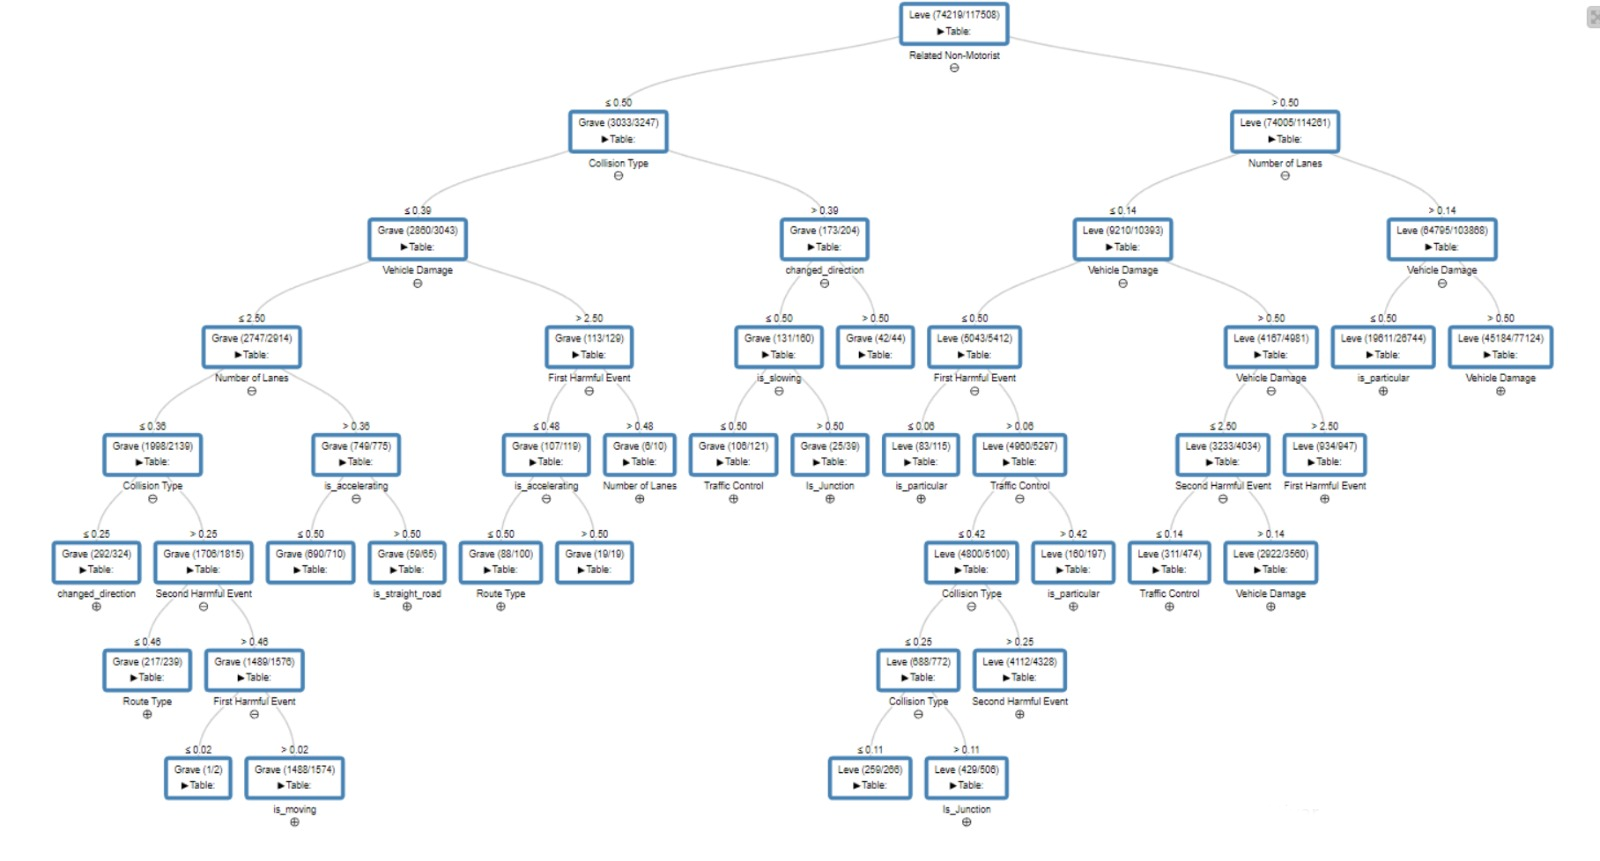
\includegraphics[width=0.4\textwidth]{Images/decision-tree.png}}
\caption{\label{fig:decision-tree} Árvore de decisão gerada usando o Knime}
\end{figure}

\subsection{Indução de Regras de Classificação}
A indução de regras vai trazer para nós um conjunto de regras em fórmula de E’s e OU’s, sendo utilizadas para classificar em uma determinada classe.
	Com o resultado da execução dos algoritmos indutores de regras. O primeiro o RIPPER (Repeated Incremental Pruning to Produce Error Reduction) que usa um processo iterativo de criação e refinamento de regras, com objetivo em melhor a precisão, sendo uma extensão do IREP, o segundo, o CN2(Classificação Numérica 2) também foi utilizado, sendo formulado em sua origem como uma extensão do primeiro.
	Após a execução iterativa dos algoritmos indutores de regra, obtivemos uma extensa lista de regras, algumas com muitas e outras com menos cláusulas. Também limitamos o número de cláusulas máximas que poderiam ser geradas.

% \subsection{Propensity score performance score}



\begin{table}[!ht]
    \centering
    \caption{Tabela de regras RIPPER Ruler Induction}
    \begin{tabular}{|l|l|l|l|l|l|}
    \hline
        Regra: & Clausula 1 & 2 & 3 & 4 & 5 \\ \hline
        1 & is\_particular=1 & is\_moving=1 & is\_slowing=0 & is\_accelerating=0 & ~ \\ \hline
        2 & is\_particular=1 & is\_moving=1 & CollisionType=Angle & Is\_Junction=1 & ~ \\ \hline
        3 & is\_particular=1 & is\_moving=1 & CollisionType=Outros & RoadCondition=0.0 & ~ \\ \hline
        4 & CollisionType=Angle & is\_particular=1 & RD=TWO-WAY, DIVIDED & ~ & ~ \\ \hline
        5 & is\_particular=1 & CollisionType=Outros & RoadCondition=0.0 & ~ & ~ \\ \hline
        6 & is\_moving=1 & is\_particular=1 & is\_slowing=0 & is\_accelerating=0 & SHE=VEHICLE RELATED \\ \hline
        7 & Hit\_Fixed\_Object=1 & is\_particular=1 & ~ & ~ & ~ \\ \hline
        8 & CollisionType=Angle & TrafficControl=2 & is\_particular=1 & ~ & ~ \\ \hline
        9 & is\_moving=1 & is\_particular=1 & RoadCondition=0.0 & CollisionType=Outros & RelatedNon-Motorist=0 \\ \hline
        10 & CollisionType=Angle & Is\_Junction=1 & is\_particular=1 & RelatedNon-Motorist=0 \\ \hline
    \end{tabular}
\end{table}

\begin{table}[!ht]
    \centering
    \begin{tabular}{|l|l|l|l|}
    \hline
        Regra: & Cobertura & Confiança & Lift \\ \hline
        1 & 0,409 & 0,591 & 1,420 \\ \hline
        2 & 0,141 & 0,675 & 1,620 \\ \hline
        3 & 0,175 & 0,659 & 1,582 \\ \hline
        4 & 0,107 & 0,682 & 1,638 \\ \hline
        5 & 0,190 & 0,638 & 1,532 \\ \hline
        6 & 0,078 & 0,620 & 1,489 \\ \hline
        7 & 0,128 & 0,744 & 1,786 \\ \hline
        8 & 0,124 & 0,674 & 1,619 \\ \hline
        9 & 0,169 & 0,708 & 1,700 \\ \hline
        10 & 0,144 & 0,675 & 1,621 \\ \hline
    \end{tabular}
\end{table}



Tabela: CN2 Rule Induction
\begin{table}[!ht]
    \centering
    \begin{tabular}{|l|l|l|l|}
    \hline
        Regra & Clausula 1 & 2 & 3 \\ \hline
        1 & CollisionType==Angle & TrafficControl>=2.0 & is\_slowing==0 \\ \hline
        2 & CollisionType==Outros & Is\_Junction!=0 & SurfaceConditionGroup!=Wet \\ \hline
        3 & Hit\_Fixed\_Object!=0 & SecondHarmfulEvent!=OBJECT RELATED & is\_slowing==0 \\ \hline
        4 & CollisionType==Angle & RoadDivision==TWO-WAY, DIVIDED & TrafficControl>=2.0 \\ \hline
        5 & CollisionType==Angle & TrafficControl>=2.0 & NumberofLanes>=3.0 \\ \hline
        6 & CollisionType==Angle & WeatherGroup==Clear & Light==LIGHT \\ \hline
    \end{tabular}
\end{table}

\begin{table}[!ht]
    \centering
    \begin{tabular}{|l|l|l|l|}
    \hline
        Regra & Cobertura & Confiança & Lift \\ \hline
        1 & 0,106 & 0,659 & 1,582 \\ \hline
        2 & 0,103 & 0,578 & 1,388 \\ \hline
        3 & 0,075 & 0,656 & 1,575 \\ \hline
        4 & 0,092 & 0,679 & 1,630 \\ \hline
        5 & 0,066 & 0,683 & 1,640 \\ \hline
        6 & 0,096 & 0,588 & 1,413 \\ \hline
    \end{tabular}
\end{table}



\section{Avaliação de Performance}
Para avaliar a performance do regressor logistico, foi utilizada a métrica AUC\_ROC que tem como
valor ideal 1, o valor obtido foi 0.788, mostrando que o regressor consegue distinguir bem entre
os valores possíveis da decisão binária.

\section{Conclusão}
Neste trabalho foi analisado quão significante foi o dano ao veìculo após o acidente,
técnicas como árvore de decisão e regressão logistica permitiram entender melhor a 
relação das características da base de dados com a variáveis alvos, enquanto a indução
de regras permitiu que relações que envolvem mais de uma característica fossem encontradas.



\begin{figure}[H]
    \centerline{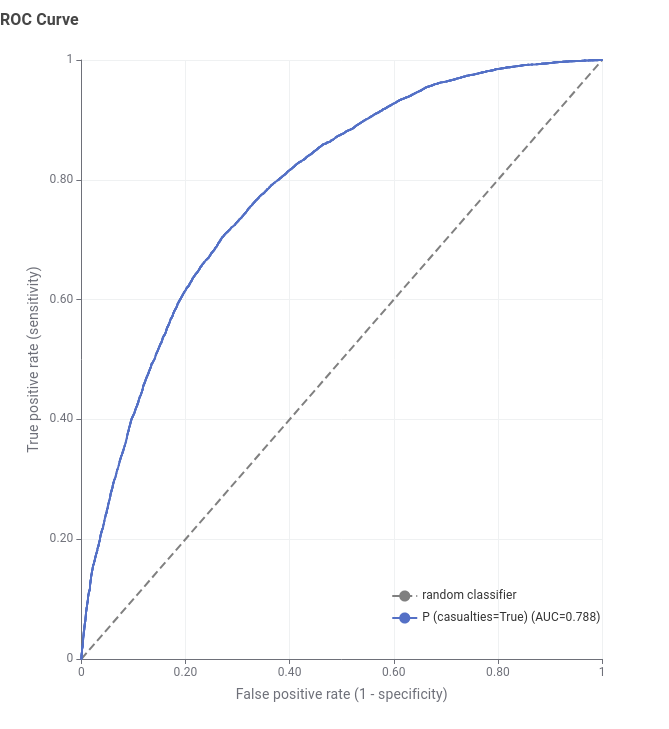
\includegraphics[width=0.4\textwidth]{Images/roc-curve-regressor.png}}
    \caption{\label{fig:decision-tree} Curva ROC Para o Regressor Logistico}
\end{figure}

\bibliography{mybib}
\nocite{*}
\bibliographystyle{IEEEtran}
\end{document}
